\section{Pruebas de rendimiento}
\label{sec:rendimiento}

\subsection{Qué se mide y qué no}

Locust mide \textbf{lo que responde la API}. Eso no dice nada sobre si el
dinero quedó bien registrado. Por eso cada carrera termina con una
verificación contra PostgreSQL que comprueba sobre los datos que la suma
global del libro mayor es cero, que ninguna cuenta está descuadrada, que
ningún saldo es negativo y cuántas transferencias quedaron realmente
escritas.

Esa última cifra da la métrica que de verdad importa, \textbf{transferencias
confirmadas por segundo}, que deja de coincidir con las peticiones por segundo
en cuanto hay fallos. La diferencia entre ambas es el resultado más
interesante de esta fase.

\subsection{Entorno}

Todas las carreras se ejecutaron en la misma máquina y en la misma sesión. El
propio script registra el entorno en cada carpeta de resultados.

\begin{table}[htbp]
\centering
\caption{Entorno de medición.}
\label{tab:entorno}
\small
\begin{tabular}{@{}ll@{}}
\toprule
CPU & AMD Ryzen 7 5800H, 16 hilos \\
Memoria & 15 GiB \\
Núcleo & Linux 7.0.0-34-generic \\
PostgreSQL & 16.10 en contenedor \\
API & Uvicorn con 4 workers, sin recarga automática \\
Generador & Locust 2.46.7, Python 3.12.3 \\
Carga & 100 usuarios, arranque de 20/s, 60 s \\
\bottomrule
\end{tabular}
\end{table}

La configuración de medición difiere de la de desarrollo en cuatro cosas,
todas deliberadas: sin recarga automática, con cuatro workers para que haya
concurrencia \emph{real entre procesos} contra PostgreSQL, con la limitación
de peticiones apagada (de lo contrario se mediría el limitador) y con el
registro a nivel \codigo{WARNING}, porque escribir una línea JSON por petición
distorsiona la latencia bajo carga.

\subsection{Escenarios}

\begin{description}[leftmargin=2.6cm,style=nextline]
  \item[\codigo{lectura}] Solo saldo e historial. Línea base: cuánto cuesta la
    infraestructura sin trabajo transaccional.
  \item[\codigo{mixto}] Lecturas y transferencias entre cincuenta cuentas al
    azar. Contención baja.
  \item[\codigo{caliente}] Todas las transferencias salen de \emph{la misma}
    cuenta. Contención máxima sobre una fila: el peor caso para el control de
    concurrencia.
\end{description}

\subsection{Resultados}

\begin{table}[htbp]
\centering
\caption{Resultados de las cinco carreras. Percentiles de
\codigo{POST /transfers}, salvo la fila de solo lectura, que corresponde a
\codigo{GET /accounts/me/balance}.}
\label{tab:rendimiento}
\scriptsize
\begin{tabular}{@{}llrrrrrrr@{}}
\toprule
\textbf{Escenario} & \textbf{Estrategia} & \textbf{Pet.} & \textbf{req/s} &
\textbf{conf./s} & \textbf{p50} & \textbf{p95} & \textbf{p99} &
\textbf{Fallos} \\
\midrule
Solo lectura & \codigo{pessimistic} & 4\,509 & 76,3 & --- &
  580 & 780 & 840 & 0,00\,\% \\
Contención baja & \codigo{pessimistic} & 4\,955 & 83,8 & 84,5 &
  590 & 770 & 990 & 0,00\,\% \\
Contención baja & \codigo{serializable} & 3\,546 & 60,0 & 43,3 &
  820 & 1\,300 & 1\,400 & 27,35\,\% \\
Contención máxima & \codigo{pessimistic} & 8\,683 & 147,0 & \textbf{148,3} &
  600 & 900 & 1\,100 & 0,00\,\% \\
Contención máxima & \codigo{serializable} & 3\,729 & 63,1 & \textbf{10,4} &
  1\,500 & 1\,900 & 2\,200 & 83,72\,\% \\
\bottomrule
\end{tabular}

\vspace{0.4em}
{\footnotesize Latencias en milisegundos. La columna \emph{conf./s} son
transferencias confirmadas por segundo, contadas en PostgreSQL. Los
percentiles los aproxima Locust por agrupación en intervalos.}
\end{table}

\begin{figure}[htbp]
\centering
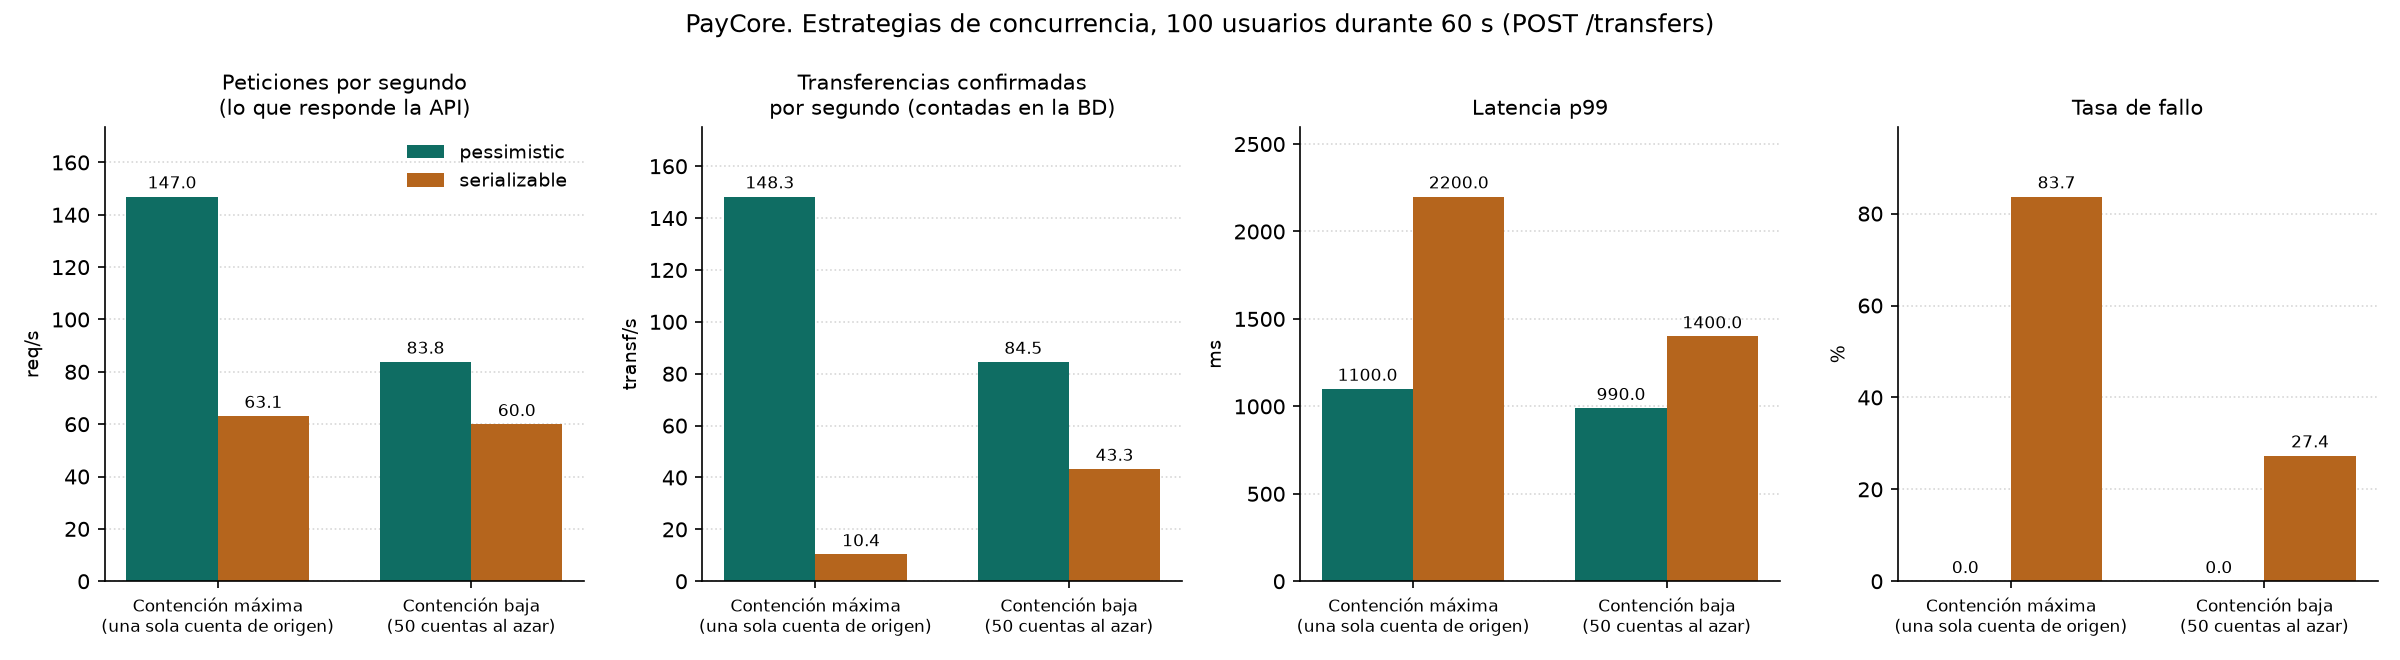
\includegraphics[width=\textwidth]{../diagrams/rendimiento-estrategias.png}
\caption{Estrategias de concurrencia bajo cien usuarios durante sesenta
segundos. El segundo panel es el que cuenta el trabajo realmente hecho.}
\label{fig:estrategias}
\end{figure}

\begin{figure}[htbp]
\centering
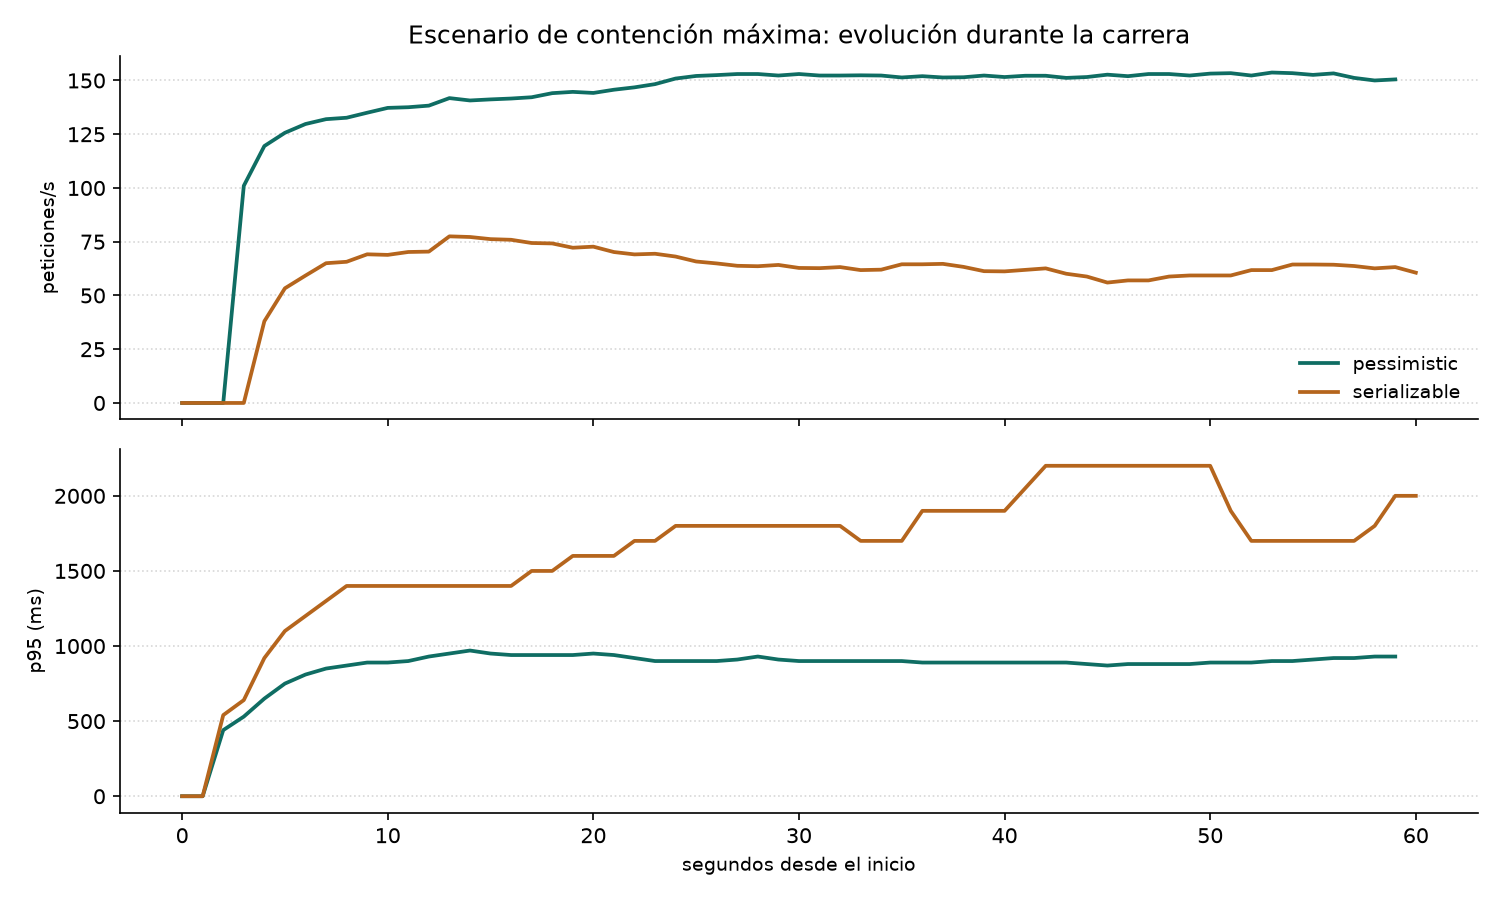
\includegraphics[width=\textwidth]{../diagrams/rendimiento-serie-temporal.png}
\caption{Evolución durante la carrera en el escenario de contención máxima.
Las dos estrategias alcanzan su régimen estacionario en los primeros segundos
y se mantienen: no hay degradación progresiva ni fuga de conexiones.}
\label{fig:serie}
\end{figure}

\subsection{Una optimización medida antes y después}
\label{subsec:optimizacion}

\paragraph{El síntoma.} La carrera de solo lectura daba menos peticiones por
segundo que el escenario mixto, que hace más trabajo, con fallos y un
percentil 95 de 30\,000\,ms. El registro señalaba la causa sin ambigüedad:
\codigo{QueuePool limit of size 10 overflow 10 reached, connection timed out,
timeout 30.00}.

\paragraph{Primera capa del diagnóstico.} Los endpoints son síncronos, así
que se ejecutan en el grupo de hilos de AnyIO, que por defecto admite cuarenta
simultáneos, mientras que el pool de cada worker entregaba como mucho veinte
conexiones. El límite de concurrencia de la aplicación y la capacidad del pool
eran dos números fijados por separado que deberían haber sido el mismo. Se
igualaron en el arranque y se bajó el tiempo de espera del pool a cinco
segundos, para fallar rápido con un 503 en lugar de dejar al cliente colgado
medio minuto. \textbf{No bastó.}

\paragraph{Segunda capa, la de verdad.} La sesión de base de datos se obtenía
como \emph{dependencia del framework}. Una dependencia se abre antes de entrar
en la función y se cierra después de salir, por lo que la conexión queda
retenida en tramos en los que la petición ya no ocupa ningún hilo. El número
de conexiones en uso podía por tanto superar al de hilos activos. La
corrección fue acotar la sesión al cuerpo del endpoint con un gestor de
contexto, de modo que cada conexión vive exactamente lo que vive su hilo.

\begin{table}[htbp]
\centering
\caption{Efecto de acotar la sesión al cuerpo del endpoint. Las dos carreras
se hicieron seguidas, con 59 s reales cada una y la misma carga.}
\label{tab:optimizacion}
\small
\begin{tabular}{@{}lrr@{}}
\toprule
\textbf{Métrica} & \textbf{Antes} & \textbf{Después} \\
\midrule
\codigo{GET /accounts/me/balance}, peticiones/s & 8,8 & 76,3 \\
Agregado de los dos endpoints de lectura & 20,8 & 154,6 \\
p50 & 270 ms & 580 ms \\
p95 & 30\,000 ms & 780 ms \\
p99 & 31\,000 ms & 840 ms \\
Máximo observado & 30\,664 ms & 1\,100 ms \\
Tasa de fallo & 3,25\,\% & 0,00\,\% \\
\bottomrule
\end{tabular}
\end{table}

\begin{figure}[htbp]
\centering
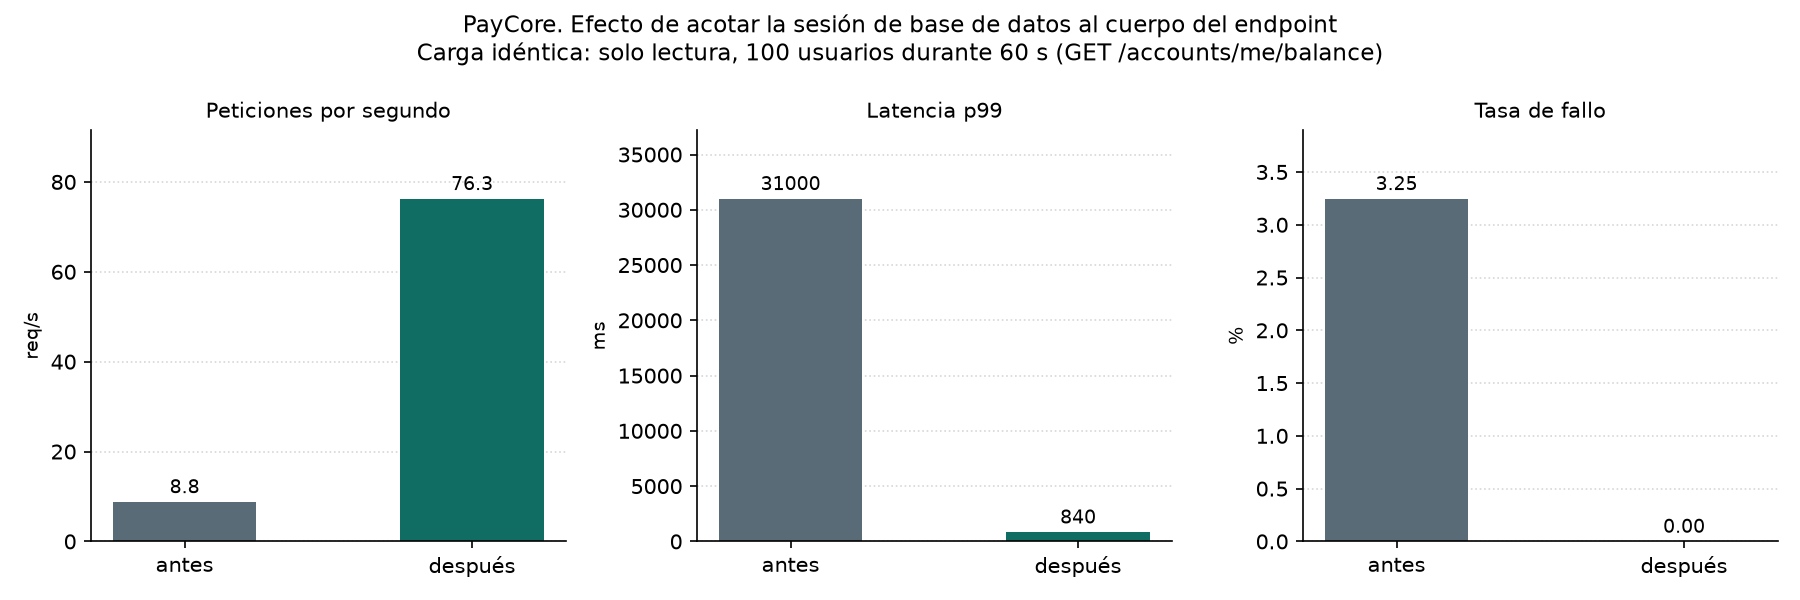
\includegraphics[width=\textwidth]{../diagrams/rendimiento-optimizacion.png}
\caption{Antes y después de la corrección, con carga idéntica.}
\label{fig:optimizacion}
\end{figure}

El rendimiento agregado se multiplica por 7,4 y la cola desaparece. Merece la
pena mirar el p50, que \textbf{sube} de 270 a 580\,ms: no es un empeoramiento,
es lo que ocurre cuando el sistema deja de descartar trabajo. Antes la mediana
solo medía a las pocas peticiones afortunadas que conseguían conexión enseguida
mientras el resto se atascaba o fallaba. Es justo el motivo por el que este
informe reporta percentiles y nunca la media sola.

\subsection{Una medición que hubo que descartar}

El primer intento de esta comparación no era válido y no se publica. La
carrera del \enquote{antes} había durado \textbf{34 segundos y no 60}, porque
el generador de carga de entonces abortaba la ejecución cuando fallaba un
inicio de sesión. Las peticiones por segundo que reportó la consola y las que
quedaron en el CSV ni siquiera coincidían entre sí, precisamente porque se
calculaban sobre ventanas de tiempo distintas de una carrera truncada.

Se detectó al comprobar las marcas de tiempo del historial antes de escribir
esta sección. Se corrigió el generador para que un inicio de sesión fallido
sea un dato y no un motivo de aborto, y se repitió la medición completa. Queda
anotado porque una cifra que no se puede defender es peor que no tener cifra.
